\chapter{Control analysis of the DNA repair rate}
%
%%\documentclass[a4paper, 12pt]{article}
%%\usepackage[english]{babel}
%%\usepackage{graphicx}
%%\makeatletter
%%\def\ScaleIfNeeded{%
%%	\ifdim\Gin@nat@width>\linewidth
%%		\linewidth
%%	\else
%%		\Gin@nat@width
%%	\fi
%%}
%%\makeatother
%%\def\TCop{\textsuperscript{\textcopyright}}
%%\def\TReg{\textsuperscript{\textregistered}}
%%\def\TTra{\textsuperscript{\texttrademark}}
%%\usepackage[applemac]{inputenc}
%%\usepackage{color}
%%\usepackage{cite}
%%\pagestyle{headings}
%
%%\newpage
%%\usepackage[T1]{fontenc}
%%\newcommand{\changefont}[3]{
%%\fontfamily{#1} \fontseries{#2} \fontshape{#3} \selectfont}
%%\changefont{phv}{m}{n}
%%\begin{document}
%\section{Introduction}

- summarize the data that we acquired
- point out that it is single cell data
- state that in image 2.5 we see a large variability of EdU kinetics 
- want to answer the question how does this slow repair arise from the molecular mechanism 
- what is the origin of the observed variability

\section{Kinetic NER model predicts collective rate control}



\subsection{Small and balanced control coefficients}
\begin{figure}[htbp]
	\begin{center}
		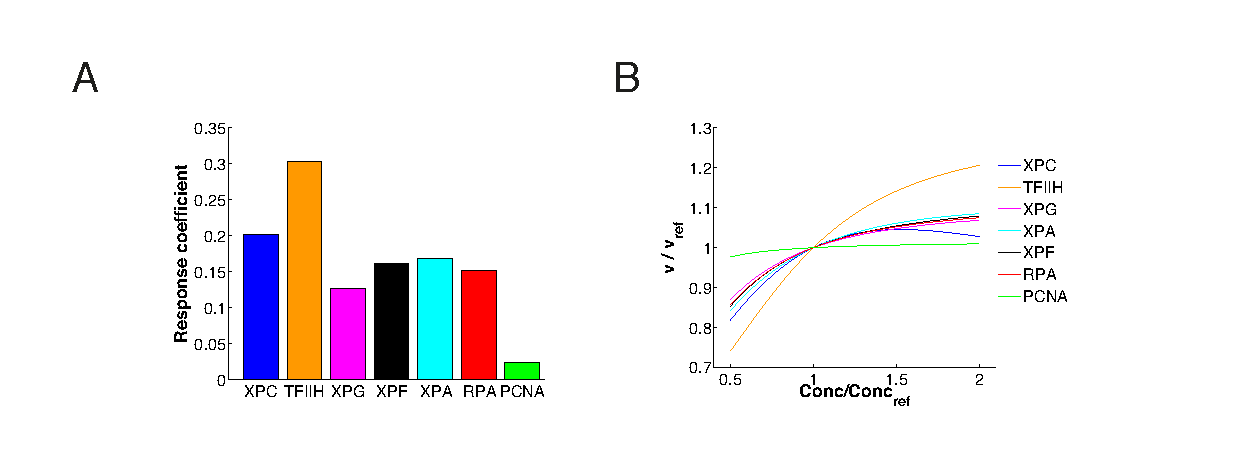
\includegraphics[width=1\textwidth]{Abbildungen/figure3_1.pdf}
		\caption{\textbf{Blubb.} A) B) }
		\label{fig:controlCoefficients}
	\end{center}
\end{figure}


\subsection{Exploiting natural variability in protein expression to quantify rate control}
\begin{figure}[htbp]
	\begin{center}
		\includegraphics[width=1\textwidth]{Abbildungen/figure3_2.pdf}
		\caption{\textbf{Blubb.} A) B) }
		\label{fig:ProteinDist}
	\end{center}
\end{figure}

\begin{figure}[htbp]
	\begin{center}
		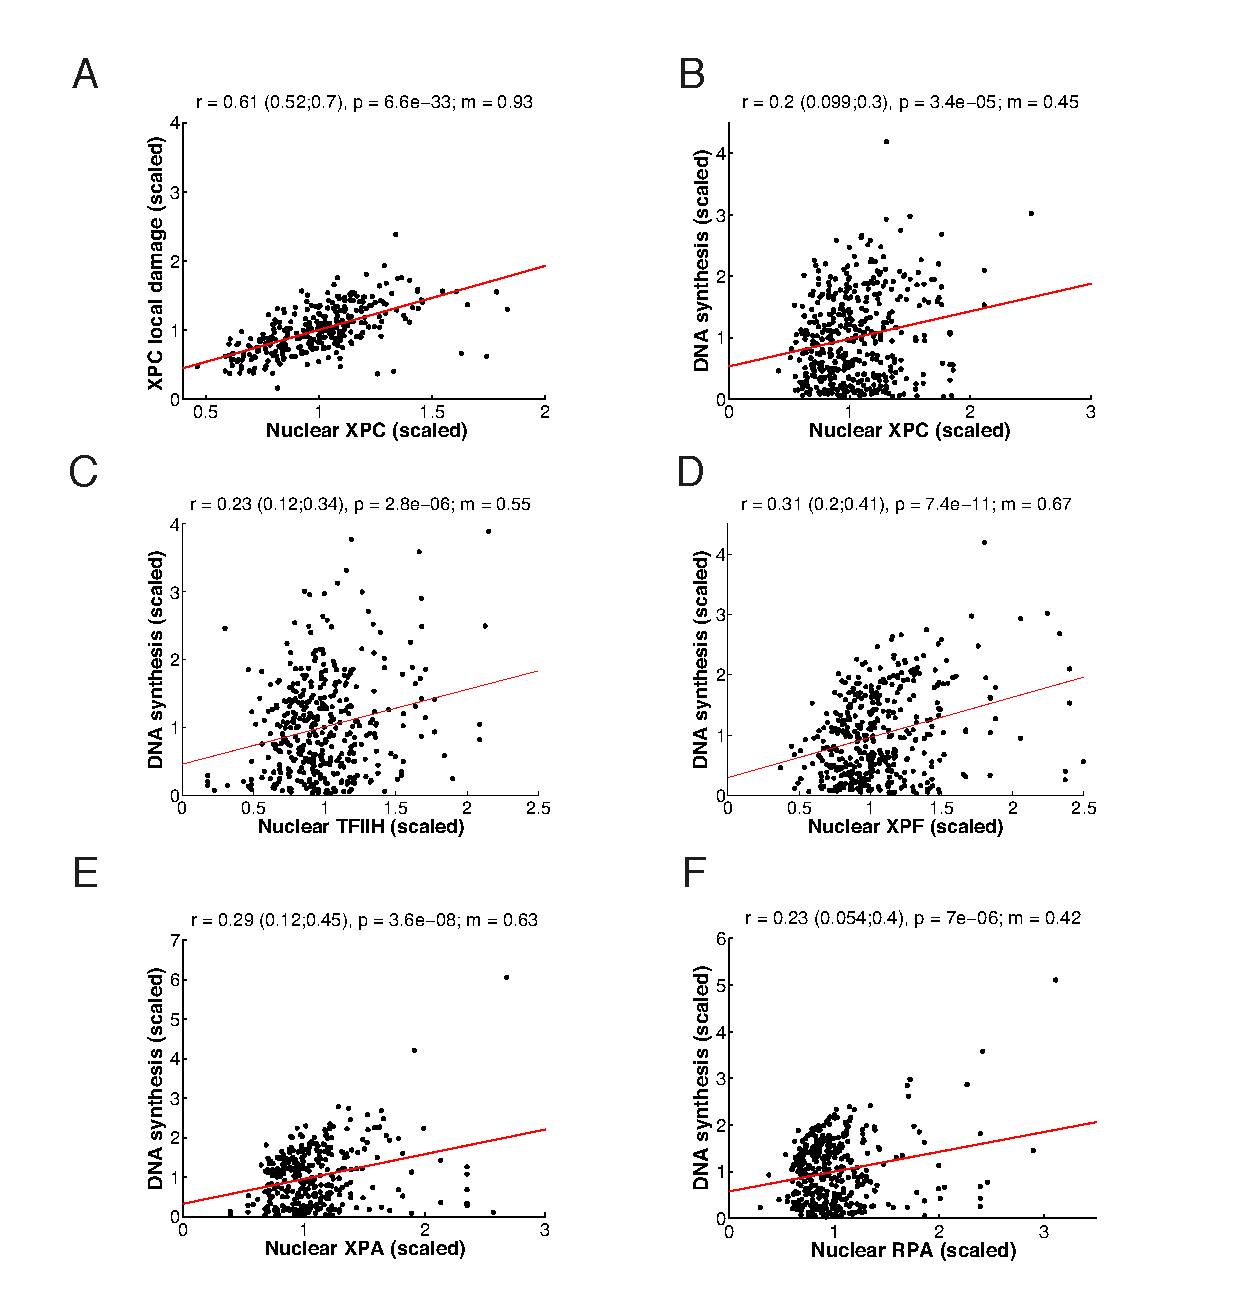
\includegraphics[width=1\textwidth]{Abbildungen/figure3_3.pdf}
		\caption{\textbf{Blubb.} A) B) }
		\label{fig:Nuc_vs_DNAsynthesis}
	\end{center}
\end{figure}

\section{Sources for repair rate variability}


\subsection{NER Variability comparable between complemented patient cell lines and native repair } 
\begin{figure}[htbp]
	\begin{center}
		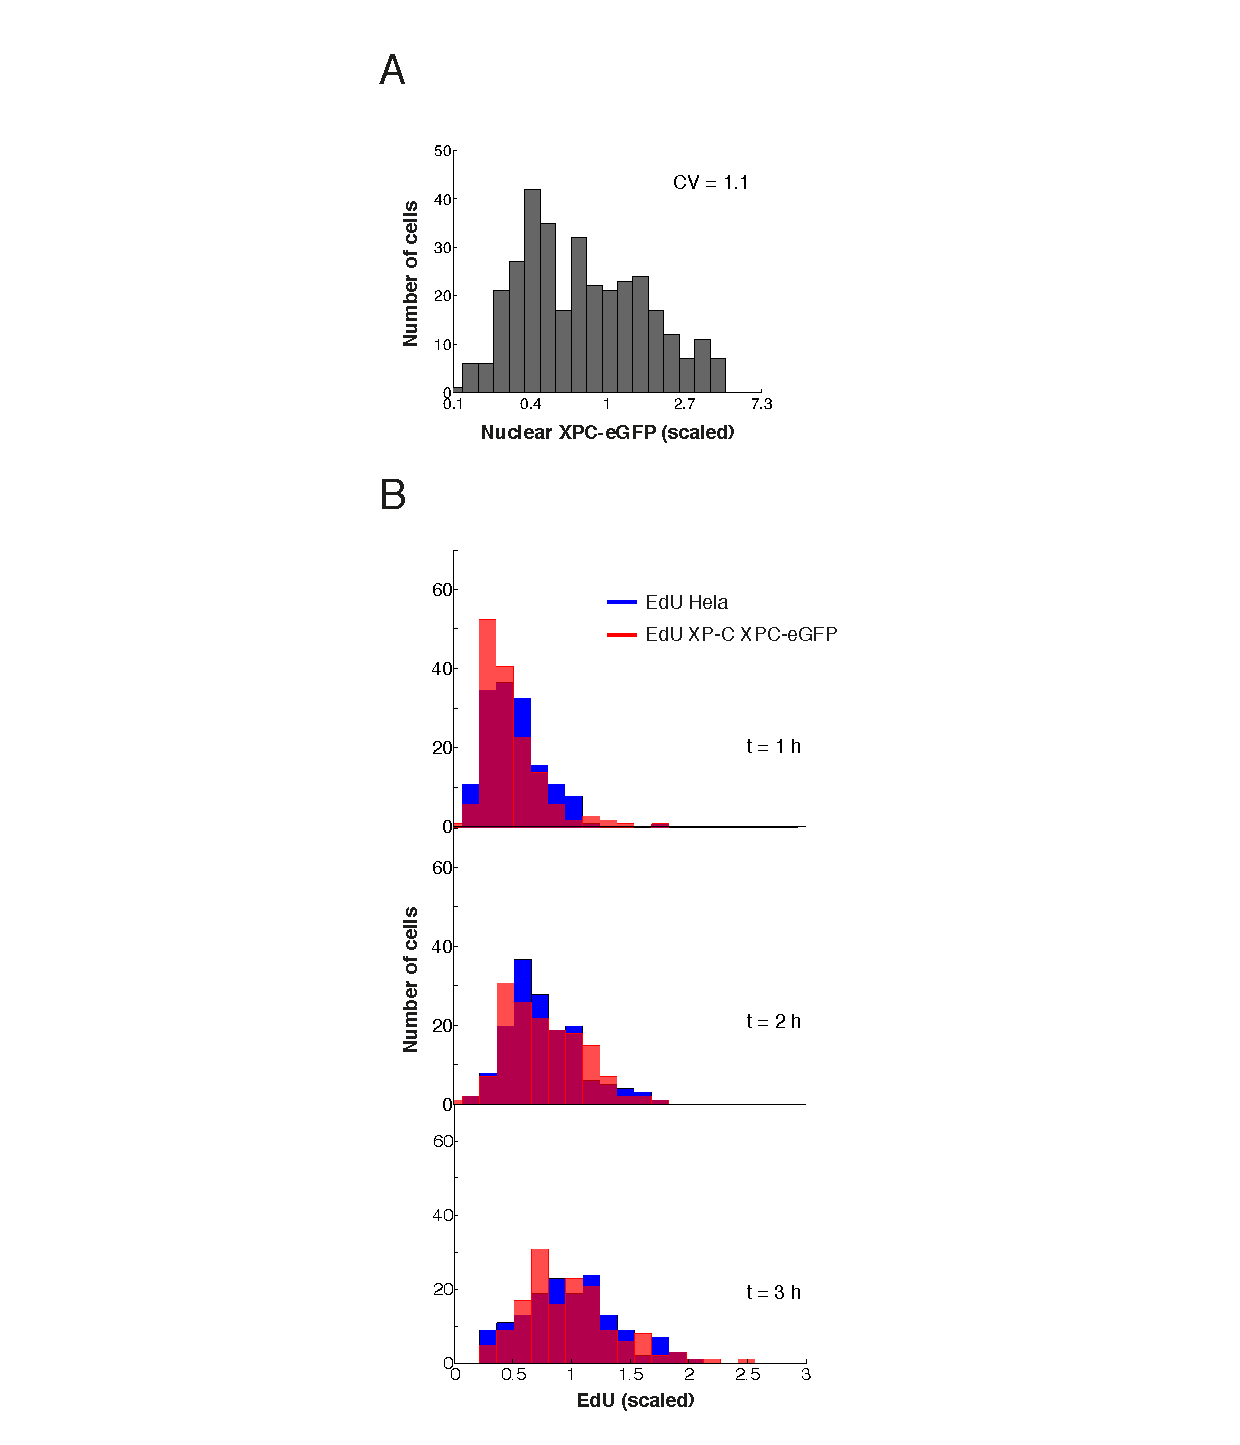
\includegraphics[width=1\textwidth]{Abbildungen/figure3_4.pdf}
		\caption{\textbf{Blubb.} A) B) }
		\label{fig:consistVariability}
	\end{center}
\end{figure}

\subsection{Variable NER factor expression and inflicted lesions account for the distribution of repair rates} 
\begin{figure}[htbp]
	\begin{center}
		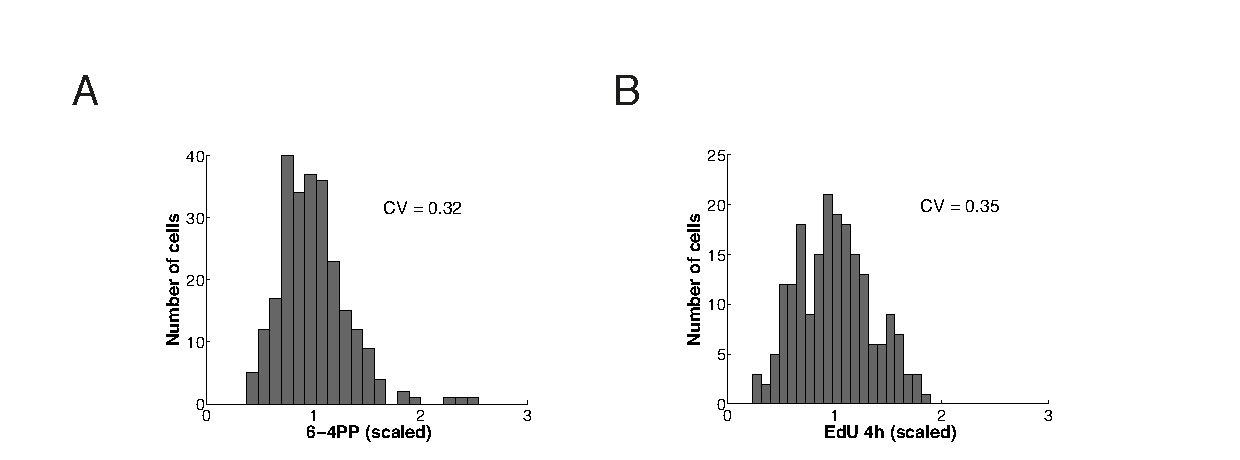
\includegraphics[width=1\textwidth]{Abbildungen/figure3_5.pdf}
		\caption{\textbf{Blubb.} A) B) }
		\label{fig:DamageDist}
	\end{center}
\end{figure}

\begin{figure}[htbp]
	\begin{center}
		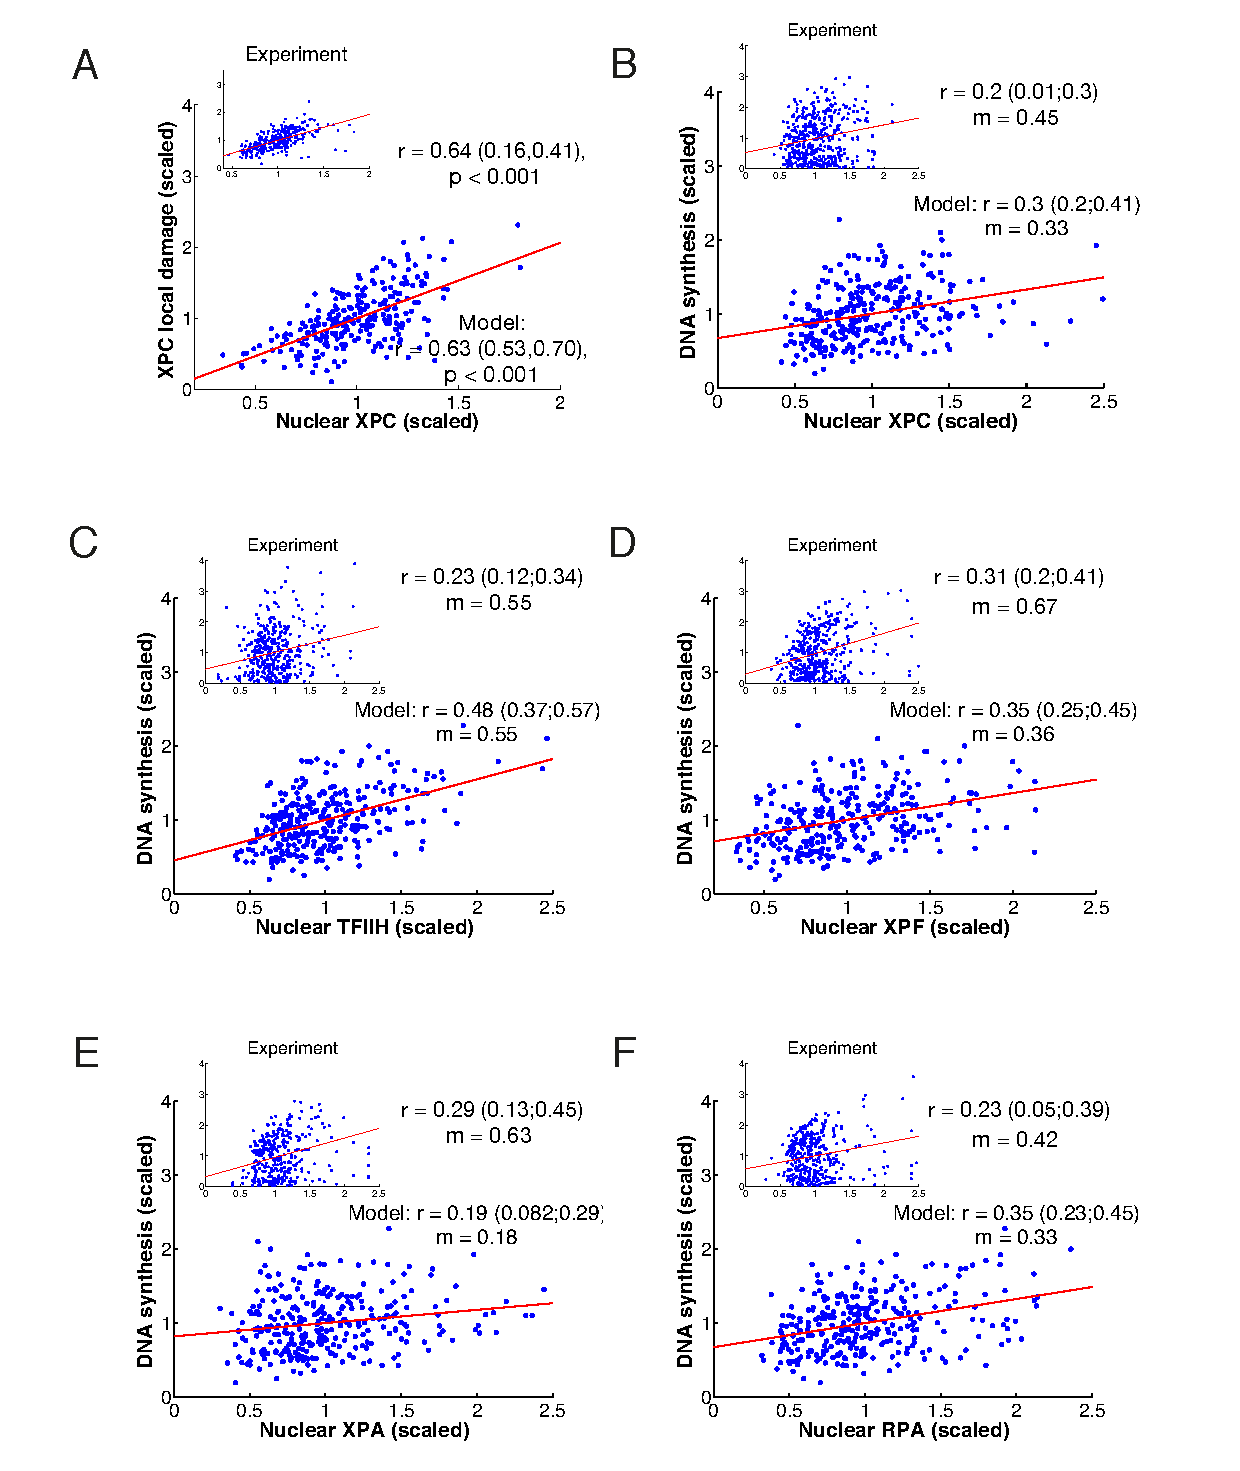
\includegraphics[width=1\textwidth]{Abbildungen/figure3_6.pdf}
		\caption{\textbf{Blubb.} A) B) }
		\label{fig:Model_dataComp}
	\end{center}
\end{figure}

\begin{figure}[htbp]
	\begin{center}
		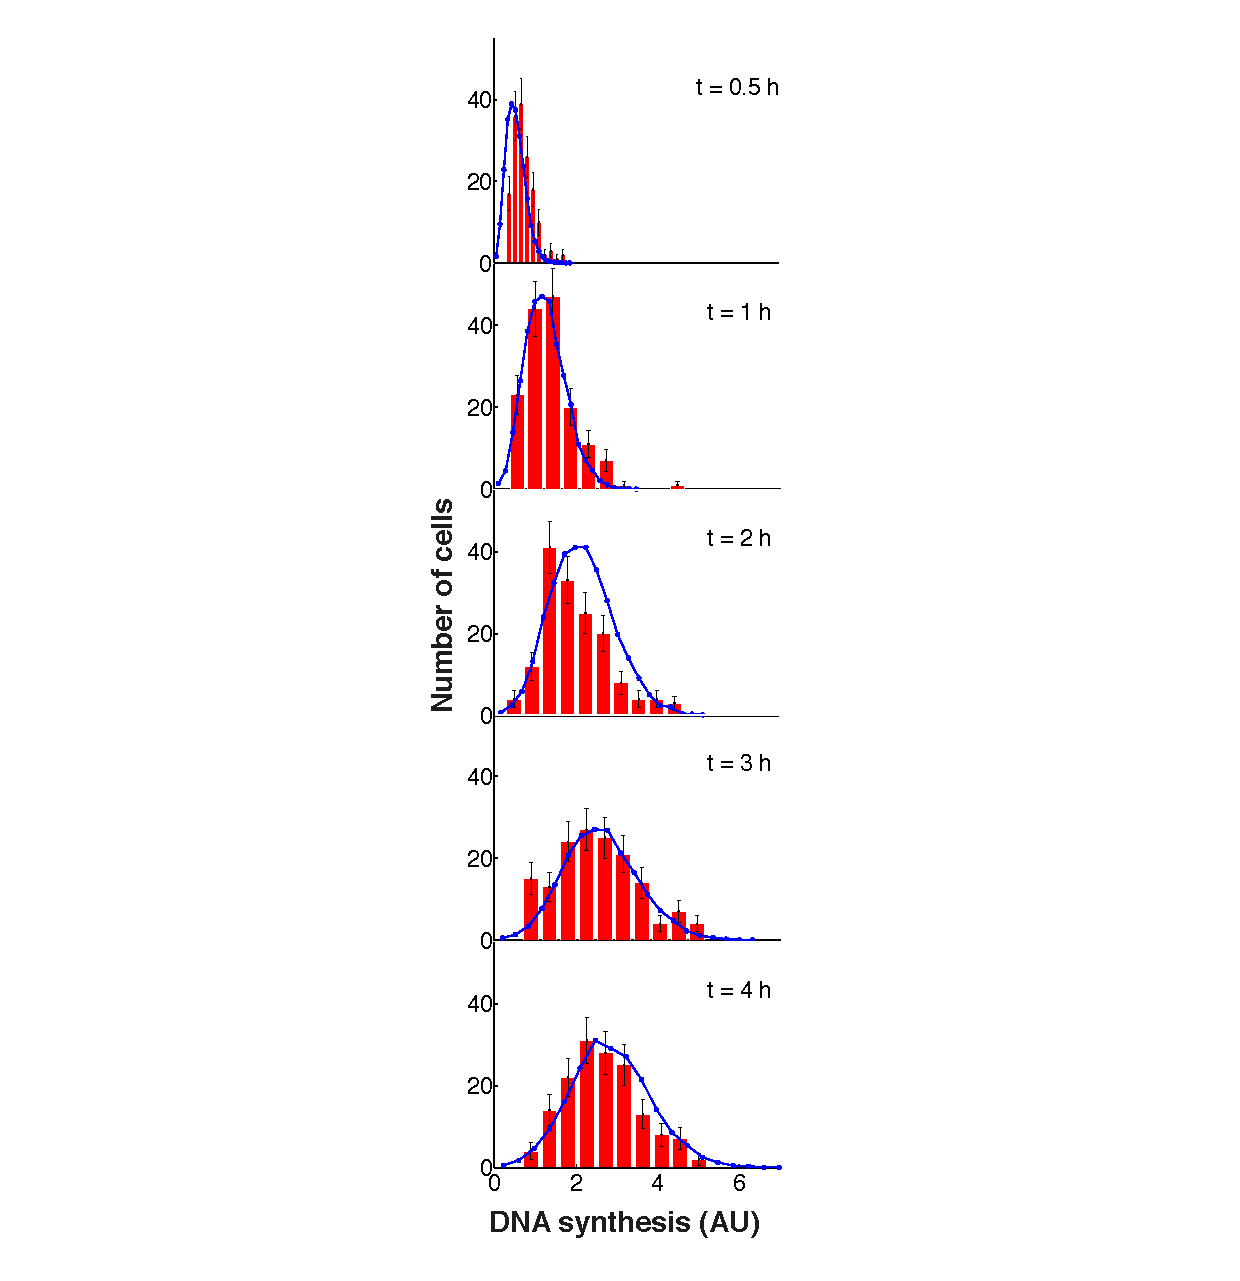
\includegraphics[width=1\textwidth]{Abbildungen/figure3_7.pdf}
		\caption{\textbf{Blubb.} A) B) }
		\label{fig:ModelData_tempVar}
	\end{center}
\end{figure}
\subsection{Imbalanced contribution }

\begin{figure}[htbp]
	\begin{center}
		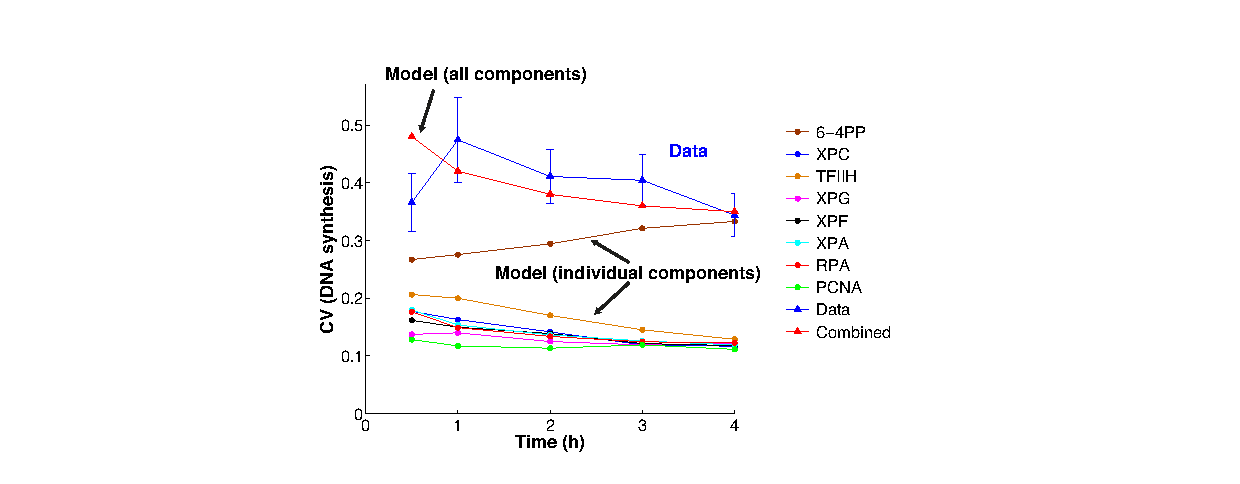
\includegraphics[width=1\textwidth]{Abbildungen/figure3_8.pdf}
		\caption{\textbf{Blubb.} A) B) }
		\label{fig:CV_Var_comp}
	\end{center}
\end{figure}
